%%%%%%%%%%%% packages %%%%%%%%%%%%%%%%%%%%%%%%%%
\documentclass[hidelinks]{article}
\usepackage[letterpaper,margin=1.0in]{geometry}
\usepackage[utf8]{inputenc}
\pagenumbering{arabic}
\usepackage{authblk}
\usepackage{graphicx}
\usepackage[singlelinecheck=false]{caption} % singlelinecheck makes single line caption left aligned instead of centered
\usepackage{subcaption}
\usepackage{amsmath}
\usepackage[round]{natbib}
\usepackage{fancyhdr}
\usepackage{longtable}
\usepackage{booktabs}

\pagestyle{fancy}
\fancyhead[R]{\textbf{On population genomic simulations of new model and non-model species: a guide}}
% for figures
\usepackage{graphicx}
\graphicspath{ {Figures/} }


% for highlighting text
\usepackage{xcolor}
\usepackage{soul}

% bibliography
\usepackage[round]{natbib}   % omit 'round' option if you prefer square brackets
\bibliographystyle{plainnat}

% hyperlinks
\usepackage{hyperref}



%commands to format figure and table references in the supplement
\newcommand{\beginsupplement}{%
        \fancyhead[L]{Supplemental Material}
        \setcounter{table}{0}
        \renewcommand{\thetable}{S\arabic{table}}%
        \setcounter{figure}{0}
        \renewcommand{\thefigure}{S\arabic{figure}}%
     }
\newcommand{\stopsupplement}{%
        \setcounter{table}{0}
        \renewcommand{\thetable}{\arabic{table}}%
        \setcounter{figure}{0}
        \renewcommand{\thefigure}{\arabic{figure}}%
     }


% Avoid pandoc bug when there are lists in the body.
\providecommand{\tightlist}{%
\setlength{\itemsep}{0pt}\setlength{\parskip}{0pt}}

\title{Adding species to the stdpopsim library}
\author[1]{M. Elise Lauterbur}
\author[2]{Maria Izabel A. Cavassim}
\author[3]{Ariella L. Gladstein}
\author[4]{Graham Gower}
\author[5]{Georgia Tsambos}
\author[6,7]{Jeff Adrion} % moved from above at request
\author[8]{Arjun Biddanda}
% \author[6]{Saurabh Belsare}
% \author[6]{Victoria Caudill}
\author[9]{Jean Cury}
\author[10]{Ignacio Echevarria}
\author[11,11]{Ahmed Hasan}
\author[13,13]{Xin Huang}
\author[15]{Leonardo Nicola Martin Iasi} % lastname Iasi
\author[16]{Jana Obšteter}
\author[17]{Vitor Antonio Corrêa Pavinato} % lastname Pavinato
\author[18,16]{David Peede}
% \author[]{Ekaterina Noskova}
% \author[]{Alice Pearson}
\author[20]{Manolo Perez}
\author[6]{Chris Smith}
\author[21]{Jeff Spence}
\author[6]{Anastasia Teterina}
\author[22]{Per Unneberg}
\author[23]{Juan Manuel Vasquez}
\author[24]{Ryan Waples}
\author[25]{Anthony Wilder Wohns}
\author[26]{Yan Wong}
\author[27]{Reed Cartwright}
\author[28]{Aaron Ragsdale}
\author[29]{Franz Baumdicker}
\author[30]{Gregor Gorjanc}
\author[31]{Ryan Gutenkunst}
\author[26]{Jerome Kelleher}
\author[6]{Andy Kern}
\author[6,32]{Peter Ralph}
\author[33]{Dan Schrider}
\author[34]{Ilan Gronau}


\affil[1]{\small{Department of Ecology and Evolutionary Biology, University of Arizona, Tucson AZ 85719}}
\affil[2]{\small{Department of Ecology and Evolutionary Biology University of California, Los Angeles}}
\affil[3]{\small{Embark Veterinary, Inc., Boston, MA 02111, USA}}
\affil[4]{\small{Section for Molecular Ecology and Evolution, Globe Institute, University of Copenhagen, Denmark}}
\affil[5]{\small{School of Mathematics and Statistics, University of Melbourne, Australia}}
\affil[6]{\small{Institute of Ecology and Evolution, University of Oregon, Eugene OR 97402}}
\affil[7]{\small{Ancestry}}
\affil[8]{\small{54Gene, Inc., Washington, DC 20005, USA}}
\affil[9]{\small{Université Paris-Saclay, CNRS, INRIA, Laboratoire Interdisciplinaire des Sciences du Numérique, UMR 9015 Orsay, France}}
\affil[10]{\small{School of Life Sciences, University of Glasgow}}
\affil[11]{\small{Department of Cell and Systems Biology, University of Toronto, Toronto ON}}
\affil[12]{\small{Department of Biology, University of Toronto Mississauga, Mississauga ON}}
\affil[13]{\small{Department of Evolutionary Anthropology, University of Vienna, Djerassiplatz 1, 1030 Vienna, Austria}}
\affil[14]{\small{Human Evolution and Archaeological Sciences (HEAS), University of Vienna, Austria}}
\affil[15]{\small{Department of Evloutionary Genetics, Max Planck Institute for Evolutionary Anthropology, Leipzig, Germany}}
\affil[16]{\small{Agricultural Institute of Slovenia, Department of Animal Science, Hacquetova ulica 17, Ljubljana, Slovenia}}
\affil[17]{\small{Entomology Dept., CFAES, The Ohio State University, Wooster, Ohio}}
\affil[18]{\small{Department of Ecology and Evolutionary Biology, Brown University, Providence, RI, USA}}
\affil[19]{\small{Center for Computational Molecular Biology, Brown University, Providence, RI, USA}}
\affil[20]{\small{Department of Genetics and Evolution, Federal University of Sao Carlos, Sao Carlos 13565905, Brazil}}
\affil[21]{\small{Department of Genetics, Stanford University School of Medicine, Stanford, CA, 94305}}
\affil[22]{\small{Department of Cell and Molecular Biology, National Bioinformatics Infrastructure Sweden, Science for Life Laboratory, Uppsala University,  Husargatan 3, SE-752 37 Uppsala, Sweden}}
\affil[23]{\small{Department of Integrative Biology, University of California, Berkeley, Berkeley, CA, USA}}
\affil[24]{\small{Department of Biostatistics, University of Washington}}
\affil[25]{\small{Broad Institute of MIT and Harvard, Cambridge, MA 02142, USA}}
\affil[26]{\small{Big Data Institute, Li Ka Shing Centre for Health Information and Discovery, University of Oxford, OX3 7LF, UK}}
\affil[27]{\small{School of Life Sciences and The Biodesign Institute, Arizona State University, Tempe, AZ USA}}
\affil[28]{\small{Integrative Biology, University of Wisconsin-Madison, Madison, Wisconsin}}
\affil[29]{\small{Cluster of Excellence - Controlling Microbes to Fight Infections, Eberhard Karls Universität Tübingen, Tübingen, Baden-Württemberg, Germany}}
\affil[30]{\small{The Roslin Institute and Royal (Dick) School of Veterinary Studies, University of Edinburgh, Edinburgh EH25 9RG, UK}}
\affil[31]{\small{Molcular and Cellular Biology, University of Arizona, Tucson, Arizona 85721}}
\affil[32]{\small{Department of Mathematics, University of Oregon, Eugene OR 97402}}
\affil[33]{\small{School of Medicine - Genetics, University of North Carolina at Chapel Hill}}
\affil[34]{\small{Efi Arazi School of Computer Science, Reichman University, Herzliya, Israel}}

\date{\small{\today{}}}

\begin{document}

\maketitle


\section*{Abstract}

Simulation is a key tool in population genetics, useful for both
methods development and empirical research. An avalance of population
genomic data is in progress, as data is being generated faster than ever before with
efforts such the Earth Biogenome and its affiliated project networks.
This data, coupled with advances in estimating detailed population genetic models, has made acute the need
for more detailed simulations of a wide range of scenarios and model and non-model species.
Many empirical researchers employing population genetics wish to simulate
their study species, but do not know what information is required in order
to do so sufficiently realistically, what is sufficient realism to address
their question, or where to find this information.
In this paper we discuss the elements of a population genomic
simulation model, including the required input data to make
them a realistic characterisation of a particular species. We also discuss
common pitfalls and major considerations in choosing this input data.
Further, we describe how new species models can be integrated into the
catalog of stdpopsim, a recently-developed tool that makes it easy to simulate
complex population genetic models using up to date information.
So far stdpopsim has been limited to well characterised model species 
such as humans, chimpanzees, and \emph{Arabidopsis},
and we illustrate the process of adding a species to stdpopsim using
examples and lessons learned from a recent hackathon designed to expand the range of supported species.
Thus, this paper provides a means to expand the accessibility of population
genetic simulations to the broader empirical and development population
genetic community by serving as a tutorial in both how to
assemble the data that is required to simulate
a species, and how this information can be incorporated
into the stdpopsim catalog to make it available to everyone.


\hypertarget{introduction}{%
\section*{Introduction}\label{introduction}}

Dramatic reductions in sequencing costs are enabling the generation of
unprecedented amounts and diversity genomic data for a huge variety of species
\citep{Ellegren2014}. Ongoing efforts to systematically sequence life on
Earth by efforts such as the Earth Biogenome \citep{Lewin2022} and its
affiliated project networks (for example, Vertebrate Genomes
\citep{Rhie2021}, 10,000 Plants \citep{Cheng2018} and others, see
https://www.earthbiogenome.org/affiliated-project-networks) are
providing the backbone to facilitate enormous increases in population-level genomic data for
new model and non-model species. Methods for inferring
demographic history and natural selection from such data are also flourishing
\citep{Beichman2018}. Past methods development has justifiably focused on the
human genome, or a few key species such as \emph{Drosophila}, 
as model systems. More recently attention is being paid to
generalize methods to include important population dynamics not present
in these models, such as inbreeding \citep{Blischak2020}, skewed offspring
distributions \citep{Montano2016}, selfing (eg. as implemented in Demes
\citep{Gower2022}), and intense artificial selection \citep{MacLeod2013,
MacLeod2014}; and to realistically model individual non-model species of interest.

Simulations from population genomic models are an important component
for analysing this new data and testing these models, making them useful for both methods
development and empirical research. For example, they provide training
data for inference methods based on machine learning \citep{Schrider2018} or
Approximate Bayesian Computation \citep{Csillery2010}. They can also serve as
baselines for further analyses: for example, models incorporating
demographic history serve as null models in selection analyses
\citep{Hsieh2016a} or to seed downstream breeding program simulations
\citep{Gaynor2020}. More recently, population genomic simulations have begun
to be used to help guide conservation decisions for threatened species
\citep{Teixeira2021}.

In general, the usefulness of population genomic simulations increases
the more realistically they represent the species being simulated - that
is, as they incorporate more relevant elements of the species' biology. Important
elements include genome features such as mutation and recombination
rates that strongly affect genetic variation and haplotype structure
\citep{Nachman2002}, particularly when linked selection is important \citep{Cutter2013}. 
Furthermore, the demographic history of a
species, encompassing population sizes, divergences, and gene flow, can
dramatically affect patterns of genetic variation \citep{Teshima2006}. Thus
estimates of these and other elements are fundamentally important to the
development of simulations of species of interest. This presents
challenges not only in the coding of the simulations themselves, but in
the choice of parameter estimates to be used to shape the simulation
model.

stdpopsim is a community resource recently developed to provide easy
access to detailed population genomic simulations \citep{Adrion2020}. This
resource lowers the technical barriers to performing these simulations
and reduces the possibility of erroneous implementation of simulations
for species with published models. But so far stdpopsim has been
primarily restricted to well-characterized model species. Feedback from
stdpopsim workshops emphasized both the community desire to simulate
non-model species of interest, ideally including these in the stdpopsim catalog;
the need for a better understanding among the empirical population
genomic community of when it is practical to create a realistic
simulation of a species of interest; and which genomic elements are
necessary and how to choose relevant parameter estimates for them.

The choice of whether and how to develop population genomic
simulations for a species of interest is affected by the intended
analysis and the genomic resources and knowledge available for the
species. These choices have a major impact on the resulting patterns of
genomic variation generated by the simulation. The fundamental
importance of these components of realistic population genomic
simulations is not always well understood, and the necessary choices can
be challenging. While stdpopsim provides a framework for standardizing
simulations of some species, the broader population genetics community
can benefit from additional guidance in making and implementing these
choices to simulate a species of interest.

Therefore this paper is intended as a resource for both methods
developers and empirical researchers to develop simulations of their own
species of interest, with the potential to submit the simulation
framework for inclusion in the stdpopsim catalog for peer review and
community use. In the \textbf{Tutorial}, we discuss the elements of a
population genomic simulation model that realistically characterizes a
species, including when a whole-genome simulation is more useful than
locus-specific or generic simulations, the required input data (genome
assembly, mutation and recombination rates, and demographic model) and
its quality, common pitfalls in choosing appropriate parameters, and
considerations for how to approach species that are missing some
necessary inputs. This paper is not intended as a tutorial for
implementing simulations in any particular simulator, rather to provide
guidance for what information is sufficient for a realistic simulation
using any simulator. We also discuss the \textbf{Application} of these
principles to modeling a species new to the stdpopsim catalog, and how
species models may be integrated into the stdpopsim catalog. This includes
briefly presenting the current method for adding species, clarifying the
required genomic resources, and describing the quality control process
that reflects the peer review of a species model.

\hypertarget{tutorial}{%
\section*{Tutorial}\label{tutorial}}

Simulation is one of the key tools in population genetics, but can
present unexpected challenges and has many hidden pitfalls for the
unwary population geneticist. Its broad use and usefulness makes it
imperative that simulations are implemented correctly at the most basic
level - the parameters describing the species. The following tutorial
presents the rationales for: 1) when whole-genome simulations meant to
realistically model a species of interest add utility beyond simple
simulations representing a few generic loci; 2) the necessary input data
with respect to the goal of the analysis; and 3) choosing what input
data to use, and when it is of sufficient quality.

\hypertarget{on-the-utility-of-simulating-the-whole-genome}{%
\subsubsection*{On the utility of simulating the whole
genome}\label{on-the-utility-of-simulating-the-whole-genome}}

When a whole-genome simulation is discussed, it can refer to simulating
one or a few chromosomes of particular interest in their entirety, or
indeed simulating all chromosomes of a species. These present different
issues, the most important of which come into play in simulating
\emph{whole chromosomes}.

It certainly seems ``more realistic'' to simulate a chromosome that
matches the real one, but strict realism is not always attainable nor
desirable. For instance, we should not ask that a simulation have
polymorphic sites at precisely the same genomic positions observed in a
real dataset, since it is these patterns of polymorphism themselves that
we want to compare to the real data. Similarly, most simulations today
do not use a reference genome sequence, since most population-level
summaries of genetic variation do not take into account nucleotide
identity. (However, this may change in the future.)

If these are elements that we do not typically seek to include for
``realism,'' what are the benefits of whole-genome simulation? While
these may vary depending on the nature of the analysis and hypotheses,
processes that have important effects on genetic diversity are central.
Primary among these is the physical linkage among sites along a chromosome. 
In biological sequences, linkage induces correlations
among nearby parts of a chromosome, even under neutral evolution. This
has multiple important consequences for simulations.

First, linkage decreases the amount of variation in a chromosome
simulated as a single continuous stretch, compared to simulating
multiple smaller fragments that add up to the same length. That is,
treating a 100Mb chromosome as 100 independent 1Mb chunks of chromosome
artificially increases the amount of independence in the data. This may
be misleading if the scale of linkage is long. For instance, results on
simulated human chromosome 22 are often very noisy due to a long stretch
of near-zero recombination \citep{Dawson2002}. The effect of natural selection
on patterns of inheritance would not have been evident if the chromosome
had been broken into many independent pieces for simulation. (TODO: I
think we lost something here - where/when would these effects not have
been evident?)

Second, linked selection, the effect of natural selection on
patterns of inheritance at nearby locations on the genome, strongly
affects patterns of genetic variation. For instance, since many types of
selection reduce diversity near the selected site(s), one might expect chromosome ends to
have increased diversity as they have less flanking sequence on which
selection might act (though other factors are in play as well). Without
using a genetic map, we can't look at the effect of linked selection on
the correlation between recombination rate and genetic diversity that is
commonly observed in practice \citep{Begun1992}. The scale over which linked
selection has an effect can differ greatly depending on the
species and the context, and the actual extent is unknown. Even in
species with large population sizes, recent selective sweeps (e.g.,
insecticide resistance \citep{Lynd2010}) can drive long haplotypes to high
frequencies.

Third, linkage has the potential to affect demographic realism. The
genetic load in a simulation of a small segment of chromosome with
deleterious mutations will necessarily be less than that in whole
chromosome. This situation makes it easy to simulate unrealistically
high levels of load without realizing it, if only unlinked segments are used.
(TODO: What is the direct effect on demographic realism of the effect of
load?)

In addition, the whole genome sequence can provide important comparative
data with which to evaluate the simulations. This is a powerful tool for
making sure the simulations correspond to the elements of biological
realism that are important for the intended analyses \citep{Hsieh2016a}. 
(@Andy and/or @Ryan, or anyone else, can you expand on this?)

Despite these potential benefits, it is much faster to simulate many
small chunks of a genome, in part because each chunk can be run
concurrently, effectively parallelizing the simulation. It is probably
safe to say that independently simulating small segments will not
introduce serious problems in some situations, but could cause serious
biases in others \citep[e.g.,][]{Nelson2020}. The degree to which it is
important to include linked selection in whole-chromosome simulations is
still a major open question.

Finally, what about \emph{whole genome} simulations? Chromosomes
segregate independently, so between-chromosome correlations are generally close
to zero. But they can be occur in fairly extreme situations, such as intense
directional or stabilising selection on multiple loci across chromosomes
\citep{Bulmer1971, Lara2022}. However, this situation can be simulated in
follow-up forward-in-time simulations \citep{Haller2018, Gaynor2020}. For
this reason, we tend to simulate chromosomes independently, and few
simulators have mechanisms to simulate
multiple chromosomes simultaneously.

\hypertarget{on-the-utility-of-working-together}{%
\subsubsection*{On the utility of working
together}\label{on-the-utility-of-working-together}}

A major advantage of the stdpopsim framework is the quality control (QC)
process, by which the parameter choices and implementation of a new
model are checked by multiple independent researchers. During this
process, the model is recreated independently by another researcher,
including decisions of parameter estimates,
without reference to the original. Any discrepancies are checked and
discussed before finalizing the model and its implementation. This
provides a mechanism to catch mistakes or points of disagreement in 
the literature and discuss alternative options
before the simulation model is used for any analyses. In our experience,
it is not uncommon to discover such mistakes or disagreements during
this process, and in fact in the published record \citep{Ragsdale2020}.

However the advantage working together to validate population genomic
model implementation is not restricted to species that are added to
the stdpopsim catalog. Researchers implementing population genomic
simulations are encouraged to have their code and parameter choices
checked by at least one other person before using it to create
simulations. In addition, basic genomic features of the simulation
results, can be compared to the reference genome and/or known population
genetic characteristics. In this too it is useful to have the input
of another researcher with fresh eyes.

\hypertarget{implementing-a-population-genomic-simulation}{%
\subsubsection*{Implementing a population genomic
simulation}\label{implementing-a-population-genomic-simulation}}

When choosing to generate appropriately realistic population genetic
simulations for a species of interest, certain population and species
genetic parameters should be known. Regardless of the simulation program used,
for analyses that benefit from whole-genome simulation (see above), 
the current standard of realism ideally includes:

\begin{enumerate}
\def\labelenumi{\arabic{enumi}.}
\tightlist
\item
  a chromosome-level \textbf{genome assembly},
\item
  an estimate of \textbf{mutation rate},
\item
  a \textbf{genetic map}, or at least an estimate of overall \textbf{recombination rate},
\item
  an estimate of \textbf{generation time},
\item
  at least one \textbf{demographic model} (or at minimum the effective
  population size of a single-population),
\item
  a \textbf{genome annotation} showing at least coding and non-coding
  regions, and
\item
  a \textbf{distribution of fitness effects} for mutations occurring in
  various annotated regions.
\end{enumerate}

Any simulation requires \emph{some} choice for 1-5, although values may
have to come from another closely-related species (though this must be
an informed, not arbitrary, choice). A fully neutral simulation does not
require genome annotation nor a distribution of fitness effects, but
these are important for simulations of selective processes. Furthermore,
all of these parameters should be documented, citeable, and
ideally chosen after discussion with another researcher.

Here we discuss all of these in more detail.

\begin{enumerate}
\def\labelenumi{\arabic{enumi}.}
\tightlist
\item
  A \textbf{genome assembly}, with contigs assembled at the chromosome
  level or nearly so. By using chromosome level information to simulate
  genomes, we can indirectly simulate the effect of linkage and linked
  selection, as discussed above. Briefly, this includes more variation
  in simulation outcomes and reduced diversity around sites of selective
  sweeps, but the length of the resulting haplotypes and effects on
  chromosome ends can vary.

Although few species currently have truly chromosome-level assemblies,
we hope that many more will be available in the near future.
This is on the horizon thanks to the advent of long-read sequencing technologies
\citep{Amarasinghe2020} and genome initiatives such as the Earth Biogenome
\citep{Lewin2022} and its affiliated project networks (for example,
Vertebrate Genomes \citep{Rhie2021}, 10,000 Plants \citep{Cheng2018} and others,
see https://www.earthbiogenome.org/affiliated-project-networks).

\item
  It is also required that the species has a plausible and citeable
  \textbf{mutation rate} estimate. Phylogenetic mutation rate, 
  germline \emph{de-novo} mutation rate, or mutation rate
  estimates based on mutation accumulation studies are
  useful. Lacking one of these, it is common to use an estimate from
  another, closely related, species.
\item
  Since recombination also shapes the genetic diversity of genomes,
  simulations also require a \textbf{recombination rate} estimate.
  Ideally, this should be a chromosome level \textbf{recombination map}, which
  allows more precise simulation of the effect of recombination
  interference. At minimum, a citeable single recombination rate
  estimate for the whole genome is necessary. Lacking this from the species
  of interest, it is common to use a recombination rate estimate from
  another, closely related, species.
\item
  A \textbf{generation time} estimate is an important part of natural
  history that is required to translate results into real time units
  (eg. years), particularly for historical demographic models. This
  estimate is not generally an element of the simulations
  themselves because these typically work in units of generations, but
  used to adjust the simulation output.
\item
  The simulated species should have at least one citeable
  \textbf{demographic model}. This model should be appropriate for
  comparison with the intended population of study, as population
  histories can vary across the species' range. This specification of
  population history is a primary determinant of its levels of genetic
  diversity. Misspecification of a demographic model can generate highly
  unrealistic patterns of genetic variation \citep[e.g.,][]{Navascues2009}. At a
  minimum, simulations require a plausible and citeable estimate of 
  \textbf{effective population size}. A single-population simulation with a
  reasonable effective size should at least give comparable levels of
  overall genetic diversity. However, if there were sizable changes in
  effective population over time \citep{MacLeod2013}, these dynamics
  will have to be incorporated to generate meaningful patterns of
  genetic diversity.
\end{enumerate}

The above factors are sufficient for modeling neutral variation in
populations, for example to infer past migration events or population
size changes under an assumption of neutrality. However, the goal of
much population genetics work is to understand the action or
consequences of selection. Although analytical models tend to study the
effect of single loci under selection in isolation, it has been
demonstrated that the effects of linked selection can vary substantially
along the genome in many species \citep{Wolf2017}, although even the general
strength and nature of this selection is still unknown. To generate
realistic amounts of selection at many locations on the genome, the
simulator needs to know where the selected sites occur, and what is the
nature of selection on them.

\begin{enumerate}
\def\labelenumi{\arabic{enumi}.}
\setcounter{enumi}{5}
\item
  The location of these sites is conveyed by a \textbf{genome
  annotation}, such as a GFF3/GFF file containing
  information about the coordinates of coding and non-coding regions,
  and the position of specific genes.
\item
  A \textbf{distribution of fitness effects} (DFE) describes the relative
  frequencies of deleterious, neutral, and beneficial mutations. This
  distribution is important for understanding the rate of adaptive
  evolution. Not all simulators are able to incorporate this
  information, those that do include the general purpose forward-in-time
  population genetics simulator SLiM \citep{Haller2019}. The DFE,
  too, should be citeable and drawn from the species of interest or one
  that is closely related.
\end{enumerate}

\hypertarget{additional-considerations}{%
\subsubsection*{Additional
considerations}\label{additional-considerations}}

A commonly-encountered thorny issue is that estimates of some of these
parameters are interrelated with others. For instance, a published
demographic model may have been estimated assuming a generation time and
mutation rate that differ from today's understanding of the best guess
at those values. In such cases, what should be done? Naively using the
demographic model with a new estimate of mutation rate may lead to
unrealistic levels of genetic diversity. In some situations the
difference may come down to only a time scaling, so that in principle a
fitted demographic model may be translated to an equivalent one that
uses a different generation time or mutation rate. However, that process
would be opaque and fraught with potential for error.

When possible, all rate, generation time, and demographic models should
be drawn from the same study. Mixing sources is not ideal, but sometimes
necessary and should be approached with deliberation. In this situation
it is especially important to discuss these choices and their potential
consequences with other researchers. (TODO: more?)

\hypertarget{what-if-we-dont-know-everything}{%
\paragraph{What if we don't know
everything?}\label{what-if-we-dont-know-everything}}

In our experience, a commonly encountered missing ingredient for a
population genetic simulations (neutral and non-neutral) in non-model
species is a chromosome-level assembly. Many species' genome assemblies
are composed of many relatively small contigs whose relation to each
other is unknown. There are two main ways to deal with this.

One option would be to effectively treat these contigs as chromosomes,
simulating them either together (unlinked) or separately. This feels
``realistic'', as the simulated chromosomes exactly match (in length, at
least) the real data. The alternative is to leave aside such strict
matching, instead simulating an anonymous chromosome from which patterns
of genetic variation can be extracted (if important, in chunks of size
similar to the contigs). The latter is usually more realistic,
since this includes linkage between sites that share a chromosome but
may be on different real contigs. As noted, this can affect patterns of neutral genetic
diversity and perhaps more crucially, linked selection. Contig-level
assemblies are sometimes annotated, and simulations of regions around
specific genes or genomic features (eg. exons) may be of interest.
However using the precise location of genes on many, unlinked contigs is
a false precision because of the importance of modeling linked selection
across contigs. For this reason, the question of ``realism'' is most
relevant for those species having chromosome-level assemblies. In our
experience it is uncommon that a species have widely-used demographic
models but not a chromosome-level assembly.

Nonetheless, some of these ingredients will likely be missing for many
non-model species. Table 1 displays some considerations and solutions
For example, if all the parameters above are available except for a
chromosome level assembly, then one might choose to include only the
larger contigs.


% Please add the following required packages to your document preamble:
% \usepackage{booktabs}
\begin{table}[]
    \captionof{table}{Guide to missing parameters.} \label{tab:title} 
    \begin{tabular}{@{}llll@{}}
    \toprule
    Missing parameter                        & Options                                                                          & Considerations                                                                                                                                       &   \\ \midrule
    \multicolumn{1}{|l|}{Mutation rate}      & \multicolumn{1}{l|}{borrow from closest relative* with a citeable mutation rate} & \multicolumn{1}{l|}{will affect levels of polymorphism}                                                                                              &   \\ \cmidrule(r){1-3}
    \multicolumn{1}{|l|}{Recombination rate} & \multicolumn{1}{l|}{borrow from closest relative with a citeable rate}           & \multicolumn{1}{l|}{will affect patterns of selection, linkage, and linked selection}                                                                & | \\ \cmidrule(r){1-3}
    Demographic model                        & At least Ne is required and is estimable from mutation rate and genetic data     & the demographic history (e.g. bottlenecks, expansions, admixture) affects patterns of variation substantially {[}CITE{]}, a constant Ne is not ideal &   \\ \bottomrule
    \end{tabular}
\end{table}

\hypertarget{application}{%
\section*{Application}\label{application}}

stdpopsim is a community resource that makes detailed, realstic
population genomic simulations accessible \citep{Adrion2020}. When first
published, the stdpopsim catalog included 6 species: \emph{Homo
sapiens}, \emph{Pongo abelii}, \emph{Canis familiaris}, \emph{Drosophila
melanogaster}, \emph{Arabidopsis thaliana}, and \emph{Escherichia coli.}
Since then, an additional 15 species have been added,
as well as multiple demographic scenarios for \emph{Homo sapiens},
\emph{Pongo abelii}, \emph{Drosophila melanogaster}, and
\emph{Arabidopsis thaliana}. However, it had the potential to be
useful to a wider community of researchers by involving the community
in adding new model and non-model species to the catalog.
To that end, the popsim consortium has made a concerted effort to 
involve the population genetics community in adding new species 
to the stdpopsim catalog.

In April 2021, we held a ``Growing the Zoo'' hackathon 
alongside the 2021 ProbGen conference. 
The hackathon was developed in response to participant demand from a
series of ``Introduction to stdpopsim'' workshops held in December 2020 and
February 2021. These workshops had over 150 participants, many of whom
expressed a wish to add their own species of interest to stdpopsim.
These workshops were followed by a ``Growing the Zoo'' workshop in
March 2021, to prepare interested participants for the hackathon. This
workshop introduced the process of developing a new model (including
parameter choice, as described above) and adding it to the stdpopsim
code base. All members of the population genetic community who were 
familiar with the this process, either from attending the
``Growing the Zoo'' workshop or their own previous work, were invited to
the hackathon. The hackathon ultimately added 12 species models to
the stdpopsim catalog (Figure \ref{fig:tree}), and started the ball rolling on expanding the
stdpopsim catalog further. However not all species models that were started
at the hackathon were added, as we learned that there is a disconnect
between what species community members wish to simulate, and those
species that have sufficient resources for a realistic simulation.

\begin{figure}
  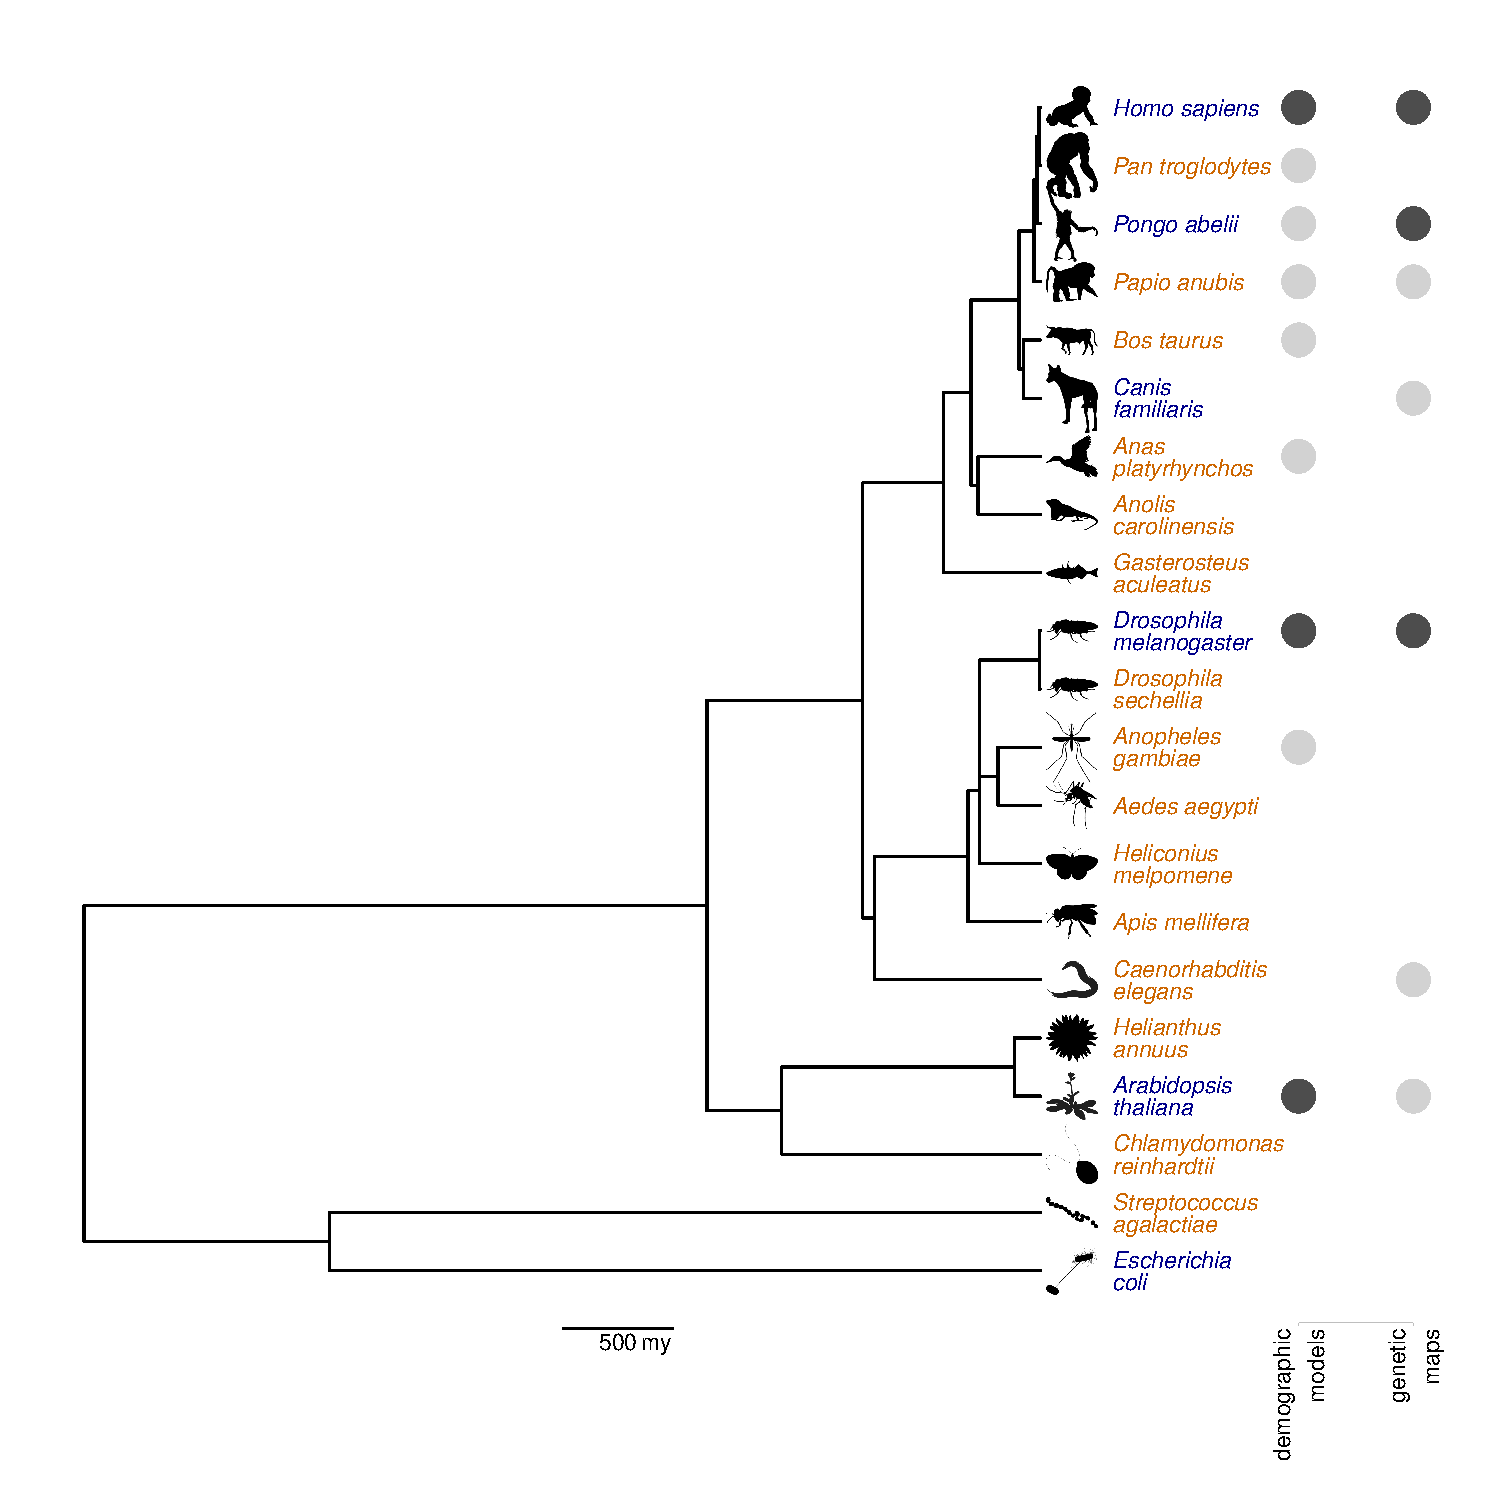
\includegraphics[width=\linewidth]{./figs/species_fig.png}
  \caption{Phylogenetic tree of species with models currently available in stdpopsim. 
           In blue are species in the original release, in orange are species added 
           by the community using the process described here.}
  \label{fig:tree}
\end{figure}

We use \emph{Bos taurus}, a species worked on during the hackathon, to
illustrate the process of choosing a species to simulate and finding and
deciding among the required resources. We also use the lessons from the
hackathon about which species are impractical to simulate to further
discuss the limitations of population genomic simulations to
realistically model species of interest when these species have
inadequate genomic resources. What it means for genomic resources to
be inadequate must be approached in the context of the research goals.

\hypertarget{examples-from-the-growing-the-zoo-hackathon}{%
\subsubsection*{Examples from the ``Growing the Zoo''
hackathon}\label{examples-from-the-growing-the-zoo-hackathon}}

\hypertarget{bos-taurus}{%
\paragraph{\texorpdfstring{\emph{Bos
taurus}}{Bos taurus}}\label{bos-taurus}}

\emph{Bos taurus} (cattle) was added to the stdpopsim catalog 
because of its agricultural importance. Agricultural species experience
strong selection due to domestication and selective breeding, leading
to a reduction in effective population size. These processes,
as well as admixture and introgression, produce patterns
of genetic variation that can be very different from typical model
species \citep{Larson2013}. In cattle, these processes have occurred over a
relatively short period (\textasciitilde 10,000 years or less) and are
increasingly intensified to improve food production \citep{Gaut2018,
MacLeod2013}. In cattle, high quality genome assemblies are now
available for several breeds \citep[e.g.,][]{Rosen2020, Heaton2021,
Talenti2022} and population genomic analyses have become widely used to
improve selective breeding and genomic prediction \citep{Meuwissen2001,
MacLeod2014, Obsteter2021}. Their small effective population size
(\textasciitilde 90 around 1980, and continuing to decline due to intense
selective breeding \citep{MacLeod2013, VanRaden2020, Makanjouloa2020}) is
challenging for demographic and selection inference \citep{MacLeod2013,
Hartfield2022} and genome-wide association and prediction
\citep{MacLeod2014}. For these reasons, it was useful to develop a
cattle model for stdpopsim.

With respect to the parameters chosen in the stdpopsim implementation,
for the basic genome simulation, we used the most recent assembly
\citep{Rosen2020}, mutation rate of \(1.2 \times 10^{-8}\) \citep{Harland2017},
recombination rate of \(0.926 \times 10^{-8}\) \citep{Ma2015}, base population
effective population of 90 \citep{MacLeod2013}, and generation interval of 5
years \citep{MacLeod2013}. The chosen effective population size is specific
to the Holstein breed, but is generally representative of a small
effective population size in other breeds. Critically, this low
effective population size will generate very low level of overall
genetic diversity, which is not in line with the actually observed
variation \citep[e.g.,][]{Rosen2020}. To remedy this, the basic genome
simulation must be complemented with a demographic model. We implemented
the \cite{MacLeod2013} demographic model for the Holstein breed, which was
inferred from runs of homozygosity in the whole-genome sequence of two
iconic bulls. The estimated effective population size in this demography
spans from the deep past (33,154 generations ago with effective population size
of 62,000) to the recent past (about 1980 with effective population size of 90),
after which further breeding simulations with intense selection breeding are
needed to reflect reality \citep[e.g.,][]{
MacLeod2014, Gaynor2020, Obsteter2021}. \cite{MacLeod2013} assumed
recombination and mutation rates of \(10^{-8}\) in inferring their
demographic model, but revised the mutation rate to \(0.94 \times 10^{-8}\) by
taking sequence errors into account. In line with the advice given in
previous sections, we implemented these mutation and recombination rates
for the \cite{MacLeod2013} demographic model, even though we have implemented
more recent estimates in the basic genome model. 
When a simulation with this demographic model is requested, stdpopsim uses the
estimates assumed in the demographic model rather than the more
recent estimates, in line with our advice of using estimates from the same
source when possible.

\hypertarget{what-about-species-lacking-chromosome-level-assemblies}{%
\paragraph{What about species lacking chromosome-level
assemblies?}\label{what-about-species-lacking-chromosome-level-assemblies}}

When we set out to cast a wide net and add a wide variety of species to
the catalog, we quickly ran into species that people were enthusiastic
to add, but lacked many (or most) of the parameters estimates discussed above. The
utility of stdpopsim is to make tricky data easily available for
simulation; such data includes genetic maps, annotations, and/or
demographic models. We have not yet encountered a species with
widely-used demographic models but no chromosome-level assembly, so the
main issue in practice seems to be around chromosome-level assemblies
and around matching genome parameters to demographic models.

However, there is no clear line for what level of assembly quality is
required to be ``useful'' - the most telling indication is whether there is
a community of users eager to use it.

\hypertarget{adding-a-species-to-stdpopsim-catalog}{%
\subsubsection*{Adding a species to stdpopsim
catalog}\label{adding-a-species-to-stdpopsim-catalog}}

In stdpopsim, once all the necessary data (Table 1) for a given species
is collected, then its inclusion is dependent upon a peer-reviewed
quality control process. Before this process, it is considered preliminary. 
If all quality control conditions are met, the
species and its simulation framework are added to the catalog. Adding a
species to the stdpopsim catalog is beneficial in many ways: (1) it
increases the visibility of the species model, (2) it drastically
improves the reproducibility of the given model framework, and (3) it
allows other researchers to test different model simulations with that
particular species.

The feedback from the workshops (2020-2021) made
it clear that many prospective users of stdpopsim want to simulate
non-model species that are not already in the stdpopsim catalog.
Currently there are multiple gaps in the species catalog (Figure \ref{fig:tree}), 
and having a greater representation of the tree of life would benefit 
the stdpopsim community as a whole.

The steps to successfully add a species to the catalog are as follow:

\begin{itemize}
\tightlist
\item
  Find citeable resources describing the required population and species
  genetic parameters as detailed in \textbf{Implementing a population genomic simulation}.
\item
  Open a GitHub account, fork the stdpopsim GitHub
  repository, and start a pull request by following the steps provided
  in the ``Adding a new species'' section of the Development chapter in
  the stdpopsim docs, currently at
  \url{https://popsim-consortium.github.io/stdpopsim-docs/stable/development.html?highlight=adding\%20species\%20catalog\#adding-a-new-species}
  These steps as they stand in April 2022 are described in detail in the
  supplementary material, but are subject to change as the stdpopsim
  framework improves.
\end{itemize}

To demonstrate the steps that it would take to add a species, here we
use the species \emph{Anopheles gambiae} (mosquito) as an example.

stdpopsim uses git for version control. Our first step will be to create an upstream
link to the version of the repository owned by
\texttt{popsim-consortium}, then we create a new branch of stdpopsim
using git to keep track of the new species model we are adding.

stdpopsim has a few utilities that interact with Ensembl \citep{ensembl2021},
including retrieving essential genome information to create code
templates for building a new species model. A partial list of the
genomes housed on Ensembl can be found at
https://metazoa.ensembl.org/species.html.

The next steps flesh out the templates, which include a directory for
the species (AnoGam, for our \emph{Anopheles gamiae} example), and three
files. These files include a data dictionary with space for the assembly
accession number, the assembly name, and the
chromosome names associated with their lengths; a file for species
specific information, including 1. \emph{chromosome-specific}
recombination rates (could also be single rate), 2. a genome-wide
average \emph{mutation rate}, 3. a \emph{generation time} estimate (in
years), 4. a default \emph{effective population size}, and 5. literature
citations that one can point to for the above and the assembly. The last
file contains the required code for stdpopsim to retrieve the species
information.

The process for adding species data requires editing the template files
with the citeable parameter choices. Here we use the recombination rate
parameter as an example. As a reference for recombination rates in
\emph{Anopheles gambiae} we use a recombination map based on a study
by \citep{Pombi2006}. In that manuscript
the authors cite rates around 1 cM/Mb, with a bit of variation among
arms. This is as easy as editing the following block of code in the
species information file (\texttt{species.py}) that defines the
recombination rate in the simulation:

\begin{verbatim}
_recombination_rate = {
    "2L": 0, # setting to zero because of inversion
    "2R": 1.3e-8,
    "3L": 1.6e-8,
    "3R": 1.3e-8,
    "X": 1e-8,
    "Mt": 0
}
\end{verbatim}

Every piece of information requires a citable reference. To include that we
can create a \texttt{stdpopsim.Citation} object in the same
\texttt{species.py} file. That object looks like this:

\begin{verbatim}
_PombiEtAl = stdpopsim.Citation(
    doi="https://doi.org/10.4269/ajtmh.2006.75.901",
    year=2006,
    author="Pombi et al.",
    reasons={stdpopsim.CiteReason.REC_RATE},
)
\end{verbatim}

stdpopsim in part guarantees code quality through the use of unit
testing, which must be run and pass before starting a pull request to
the stdpopsim github repository.

The full quality control process is fully described at
https://popsim-consortium.github.io/stdpopsim-docs/stable/development.html?highlight=adding\%20species\%20catalog\#demographic-model-review-process.
In summary, we find another stdpopsim contributor (reviewer) to conduct
the quality control process, which consists of: creating a blind
implementation of the model and species to be added; running unit tests
to verify the equivalence of the catalog and quality control model
implementations; and creating a new pull request which is then finally
merged. If conflicts arise between the original and new implementations,
these are discussed and we and the reviewer must come to an agreement.
Outside opinions are useful. Once these conflicts are resolved, the
model graduates from preliminary to a fully vetted model in the stdpopsim catalog.

It is important to note that the catalog is mutable. If more accurate
estimates for a given species are published, then chances are that the
catalog will be updated upon a new quality control review process.

\hypertarget{conclusion}{%
\section*{Conclusion}\label{conclusion}}

As our ability to sequence genomes continues to advance, the need for
population genomic simulation of new model and non-model organism genomes is
becoming acute. So too is the concomitant need for an expandable framework
for implementing such simulations and for species of interest, and
the resources for understanding when and how to do so.

In this manuscript we present the basic considerations for implementing
population genomic simulations, agnostic to simulation program. We
describe the steps of determining if a species-specific population
genomic simulation is appropriate for the species and question, what
data is necessary and why, special considerations for finding or using
that data, how to proceed when some of that data is not available,
and why we encourage everyone implementing simulations to have their
parameter choices and implementation reviewed by at least one other
researcher.

We also show how these can be integrated into the stdpopsim catalog, a
resource that is uniquely poised to fill this gap as it provides easy
access to simulation which conditions on species-specific information,
easy inclusion of new species genomes, and community-maintained accuracy
and correctness. We additionally briefly describe how the quality control 
process for species inclusion works. Currently, large-scale efforts such as the Earth Biogenome
and its affiliated project networks are generating tens of thousands of genome
assemblies. Each of these assemblies, with some prior knowledge of mutation and
recombination rates, will become a candidate for inclusion into the
stdpopsim catalog following the steps we have outlined above. As
annotation of genome assemblies improves over time those too can easily
be added to the stdpopsim catalog.

Moreover, one of the goals of stdpopsim is to leverage stdpopsim itself
as a springboard for education and inclusion of new communities into
computational biology and software development. We are keen to use
outreach, for instance in the form of workshops and hackathons, as a way
to democratize development of population genetic simulation as well as
grow the stdpopsim catalog and library generally. By enabling
researchers of non-model species with simulation platforms that
traditionally have been quite narrowly focused with respect to organism,
we hope to raise the quality of research across a large number of
systems, while simultanousely expanding the community of software
developers at work in the population and evolutionary genetics world.
Our experience with such outreach over the past two years is that people
are indeed keen to to in the time and effort to include their favority
study species, but that simple, clear guidance was the key. Our
intention with this paper is in part to provide another learning
modality to meet that need.

\hypertarget{acknowledgements}{%
\section*{Acknowledgements}\label{acknowledgements}}

TODO Workshop and hackhaton attendes?

\hypertarget{funding}{%
\section*{Funding}\label{funding}}

TODO: should we order these alphabetically or in the same order as authors?

M. Elise Lauterbur was supported by an NSF Postdoctoral Research Fellowship \#2010884.

Gregor Gorjanc was supported by the University of Edinburgh and BBSRC grant to The Roslin Institute (BBS/E/D/30002275).

Andrew D. Kern and Peter L. Ralph were supported by NIH award R01HG010774.

\bibliography{references}
\end{document}
